\documentclass[aspectratio=169, 14pt]{beamer}
\usepackage[utf8]{inputenc}
\usepackage[english]{babel}
\usepackage{tipa}
\usepackage{graphicx}
\usepackage{transparent}
\usepackage[ruled, lined, linesnumbered, commentsnumbered]{algorithm2e}
\usepackage{pgfplots}
\newcommand\mycommfont[1]{\small\ttfamily\textcolor{blue}{#1}}
\SetCommentSty{mycommfont}
\renewcommand{\thealgocf}{}
\usepackage{setspace}
\usepackage{tikz}
\usetikzlibrary{matrix,backgrounds}
\usetikzlibrary{arrows}
\usetikzlibrary {arrows.meta}
\usetikzlibrary{calc,shadows.blur,fit,positioning}
\usetikzlibrary{shapes.multipart,chains}
\usepackage{minted}
\usepackage{fontawesome5}
\usepackage{booktabs}
\usepackage{caption}
\usepackage{bookmark}
\usepackage{hyperref}
\hypersetup{
	colorlinks=true,
	linkcolor=blue,
	filecolor=magenta,
	urlcolor=cyan,
}
\urlstyle{same}
\usetheme{metropolis}
\metroset{block=fill}
\usecolortheme{default}
\definecolor{darkmidnightblue}{rgb}{0.0, 0.2, 0.4}
\definecolor{LightGray}{gray}{0.9}


%------------------------------------------------------------
%This block of code defines the information to appear in the
%Title page
\title[Data Structures] %optional
{Data Structures}

\subtitle{Python Crash Lesson \& Built-in Data Structures}

\author[CHEN Zhongpu] % (optional)
{CHEN Zhongpu}

\institute[] % (optional)
{
	School of Computing and Artificial Intelligence \\
	\href{mailto:zpchen@swufe.edu.cn}{zpchen@swufe.edu.cn}
}

\date[] % (optional)
{SWUFE, Fall 2022}

%End of title page configuration block
%------------------------------------------------------------


%------------------------------------------------------------
%The next block of commands puts the table of contents at the 
%beginning of each section and highlights the current section:

% \AtBeginSection[]
% {
%   \begin{frame}
%     \frametitle{Table of Contents}
%     \tableofcontents[currentsection]
%   \end{frame}
% }
%------------------------------------------------------------


\begin{document}

%The next statement creates the title page.
\frame{\titlepage}

%---------------------------------------------------------
%This block of code is for the table of contents after
%the title page
% \begin{frame}
% \frametitle{Table of Contents}
% \tableofcontents
% \end{frame}
%--------------------------------------------------------

{
	\usebackgroundtemplate{
		\tikz[overlay,remember picture]
		\node[opacity=0.3, at=(current page.south east),anchor=south east, yshift=2cm,xshift=4cm] {
			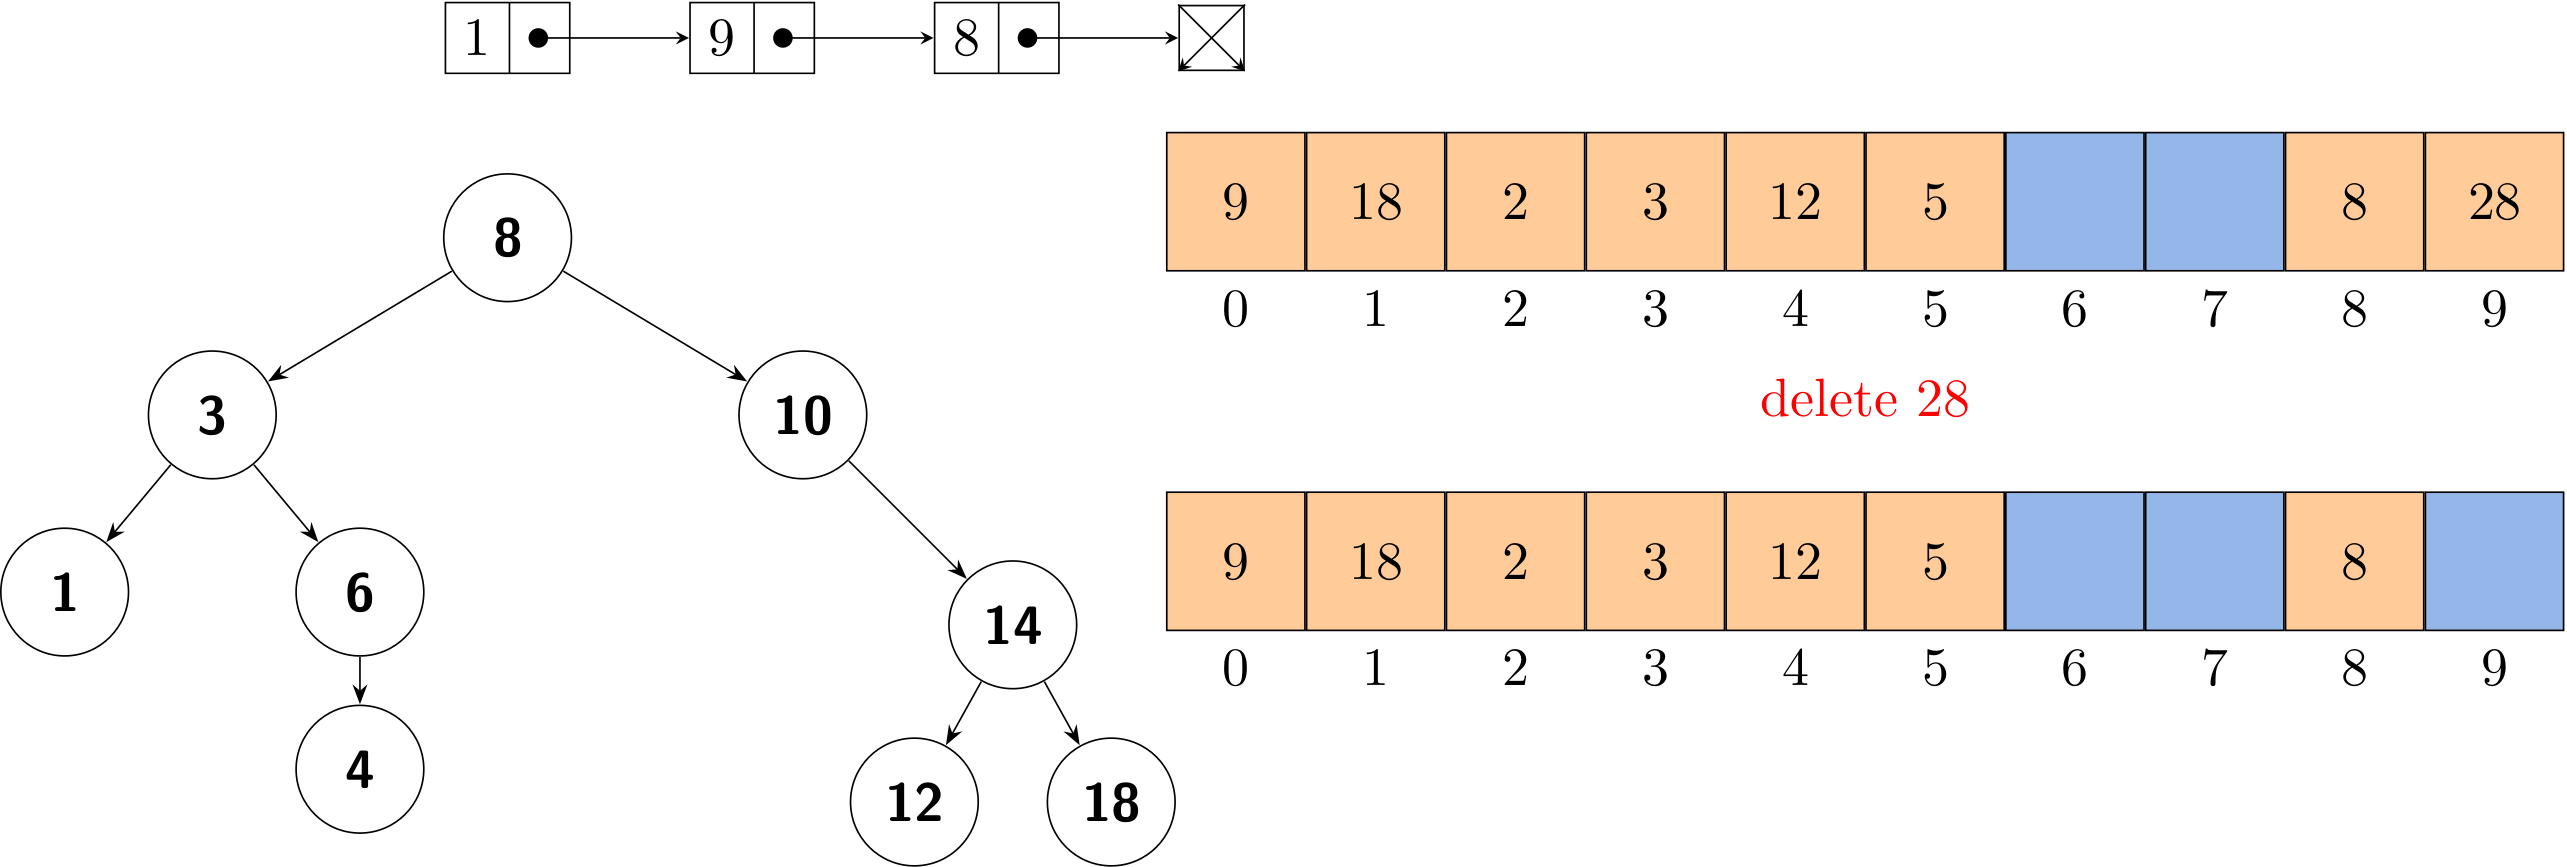
\includegraphics[height=0.6\paperheight]{cover}};
	}
	\begin{frame}
		\section{\textcolor{darkmidnightblue}{Python Crash Lesson}}
	\end{frame}
}

\begin{frame}
	\frametitle{How to learn Python}
	Recommended resources:

	\begin{itemize}
		\item \faIcon{python} Tutorial:\url{https://docs.python.org/3/tutorial/index.html}. Read through from Chapter 1 to Chapter 5, and Chapter 9.
		\item \faIcon{book} Book: Python Crash Course, 3rd Edition, by Eric Matthes.
		\item \faIcon{blog} Blog: \url{https://realpython.com/}
	\end{itemize}
	Yet another 8-week \href{https://github.com/ChenZhongPu/python-swufe}{course} by me. Note that \alert{class} (object-oriented programming) is not covered.

\end{frame}

\begin{frame}
	\frametitle{Overview of Python basics}
	There is no need for you to master every corner of Python. But you should be familiar with the following concepts:
	\begin{enumerate}
		\item \alert{Common data types}: integer, float, string, boolean, list, tuple, dictionary, set
		\item \alert{Control flows}: if-else, while, for
		\item \alert{Functions}: definition, parameters, return values
		\item \alert{Classes}: definition, method, field
	\end{enumerate}
\end{frame}

\begin{frame}[fragile]

	\begin{minted}[bgcolor=LightGray]{python}
# your first Python program
print('Hello World!')
  \end{minted}

	\begin{minted}[bgcolor=LightGray]{java}
public class Main {
    public static void main(String[] args)  {
        System.out.println("Hello World!");
    }
}
  \end{minted}
\end{frame}

\begin{frame}[fragile]
	\frametitle{Variables and types}
	In Python, every variable has a type (class). Unlike Java, integers in Python have no limit in size.
	\begin{minted}[bgcolor=LightGray]{python}
# Different from Java, Python is dynamically typed,
# and you can use type() to check its type.
i = 1 
i = 3.14
i = 'hello'
i = True
i = None
  \end{minted}

\end{frame}

\begin{frame}[fragile]
	\frametitle{Math in Python}

	\begin{minted}[bgcolor=LightGray]{python}
# / always returns a float
# // is floor division
i = 1 + 2 * 2 + 9 / 2 - 9 % 2 + 9 // 2 + 9 ** 2
i = 2 > 1
j = 2 > 1 and 3 > 2
k = 1 > 2 or 3 > 2
i = not i
  \end{minted}
\end{frame}

\begin{frame}[fragile]
	\frametitle{Control flow: if}
	\begin{minted}[bgcolor=LightGray]{java}
Scanner scanner = new Scanner(System.in);
System.out.print("Input your score: ");
float score = scanner.nextFloat();
if (score >= 65) {
    System.out.println("Pass");
} else {
    System.out.println("Fail");
}
\end{minted}
\end{frame}

\begin{frame}[fragile]

	\begin{minted}[bgcolor=LightGray]{python}
score = float(input('Input your score: '))
if score >= 65:
  print('Pass')
else:
  print('Fail')
  \end{minted}
	\alert{Indentation} is important in Python! PEP8, the official guide of Python code, suggests using \alert{4 spaces} for indentation.
\end{frame}

\begin{frame}[fragile]
	\frametitle{Exercise}
	\begin{minted}[bgcolor=LightGray, fontsize=\small]{java}
// Please translate the following Java code to Python
int i = 11, j = 8;
if (i > j) {
    System.out.println("i is greater than j");
    if (i > 10) {
        System.out.println("i is greater than 10");
    }
} else if (i == j) {
    System.out.println("i is equal to j");
} else {
    System.out.println("i is less than j");
}
  \end{minted}
\end{frame}

\begin{frame}[fragile]
	\frametitle{Control flow: while}
	\begin{block}{Example}
		To compute the result of $\sum_{i=1}^{100}{i}$.
	\end{block}

	\begin{minted}[bgcolor=LightGray,fontsize=\small]{python}
i = 1
s = 0
while i <= 100:
    s += i
    i += 1
print(s)
  \end{minted}
	Like Java, Python also has \alert{break} and \alert{continue} statements.
\end{frame}

\begin{frame}[fragile]
	\frametitle{Control flow: for}
	Python doesn't support the traditional \alert{for (int i = 0; i < n; i++)}, and it only supports \alert{for-each} loop.

	\begin{verbatim}
for item in iterable_object:
    # do something
\end{verbatim}
	For example, \alert{str} object is iterable.

	\begin{minted}[bgcolor=lightgray,fontsize=\small]{python}
university = 'swufe'
for c in university:
    print(c)
  \end{minted}
\end{frame}


\begin{frame}[fragile]

	\begin{minted}[bgcolor=lightgray,fontsize=\small]{python}
s = 0
for i in range(1, 101):
    s += i
print(i)
  \end{minted}
	\alert{range()} is a simple way to generate a sequence of numbers, which is iterable.

	\begin{tikzpicture}
		\node[fill=yellow,blur shadow={shadow xshift=-0.5ex},
			text width=20em,anchor=south west,rounded corners]
		{\faIcon{lightbulb} Always ask for \alert{help()} in Python shell.};
	\end{tikzpicture}
	\pause

	\textbf{Exercise}: Given a string, return the number of vowels.
\end{frame}

\begin{frame}[fragile]
	\frametitle{Functions}
	Strictly speaking, Java doesn't have functions, but methods. In Python, we have functions, which are defined by \alert{def} keyword.

	\begin{minted}[bgcolor=lightgray,fontsize=\small]{java}
public int add(int a, int b) {
  return a + b;
}
  \end{minted}

	\begin{minted}[bgcolor=lightgray,fontsize=\small]{python}
def add(a, b):
   return a + b
  \end{minted}

\end{frame}

\begin{frame}[fragile]

	\textbf{Example}: define a function to count the number of vowels in a string.

	\begin{minted}[bgcolor=lightgray,fontsize=\small]{python}
def count_vowels(s):
    count = 0
    for c in s:
        if c.lower() in 'aeiou':
            count += 1
    return count
  \end{minted}
\end{frame}

\begin{frame}[fragile]
	You can also specify the type of parameters and return value of a function, which is called \alert{type hint} or \alert{type annotation}.

	\begin{minted}[bgcolor=lightgray,fontsize=\small]{python}
def add(a: int, b: int) -> int:
    """To add two integers and return the result."""
    return a + b
  \end{minted}

	It is optional but recommended, because it can help you find bugs and make your code more readable.
\end{frame}

\begin{frame}[fragile]
	\frametitle{Modules}
	\begin{exampleblock}{Module}
		A module in Python is a file containing Python definitions and statements.
	\end{exampleblock}
	For example, \alert{math} is a built-in module.

	\begin{minted}[bgcolor=lightgray,fontsize=\small]{python}
import math

value = math.sin(math.pi / 2)
  \end{minted}
	You can also import specific definitions from a module, such as \alert{from math import sin}.
\end{frame}

\begin{frame}
	Python has a large standard library, which provides rich functions and modules. You can find the full list at \url{https://docs.python.org/3/library/}.

	Moreover, Python also has a large third-party library ecosystem, such as \alert{NumPy}, \alert{Pandas}, \alert{Matplotlib}, \alert{Scikit-learn}, \alert{PyTorch}, etc., which can be installed by \alert{pip} or \alert{conda}.

\end{frame}

\begin{frame}[fragile]
	\frametitle{Class}
	Every variable in Python is an object, and every object has a type, which is called \alert{class}.
	\begin{minted}[bgcolor=lightgray,fontsize=\small]{java}
class Dog {
    int age;
    String name;

    public Dog(int age, String name) {
        this.age = age;
        this.name = name;
    }
}
  \end{minted}
\end{frame}

\begin{frame}[fragile]

	\begin{minted}[bgcolor=lightgray,fontsize=\small]{python}
class Dog:
    def __init__(self, age, name):
        self.age = age
        self.name = name
# dog = Dog(2, 'Tom')
  \end{minted}

	\begin{itemize}
		\item \alert{\_\_init\_\_()} is the constructor of a class.
		\item \alert{self} is the reference to the current instance of the class, and it is the first parameter of every method.
	\end{itemize}
\end{frame}

{
\usebackgroundtemplate{
	\tikz[overlay,remember picture]
	\node[opacity=0.3, at=(current page.south east),anchor=south east, yshift=2cm,xshift=4cm] {
		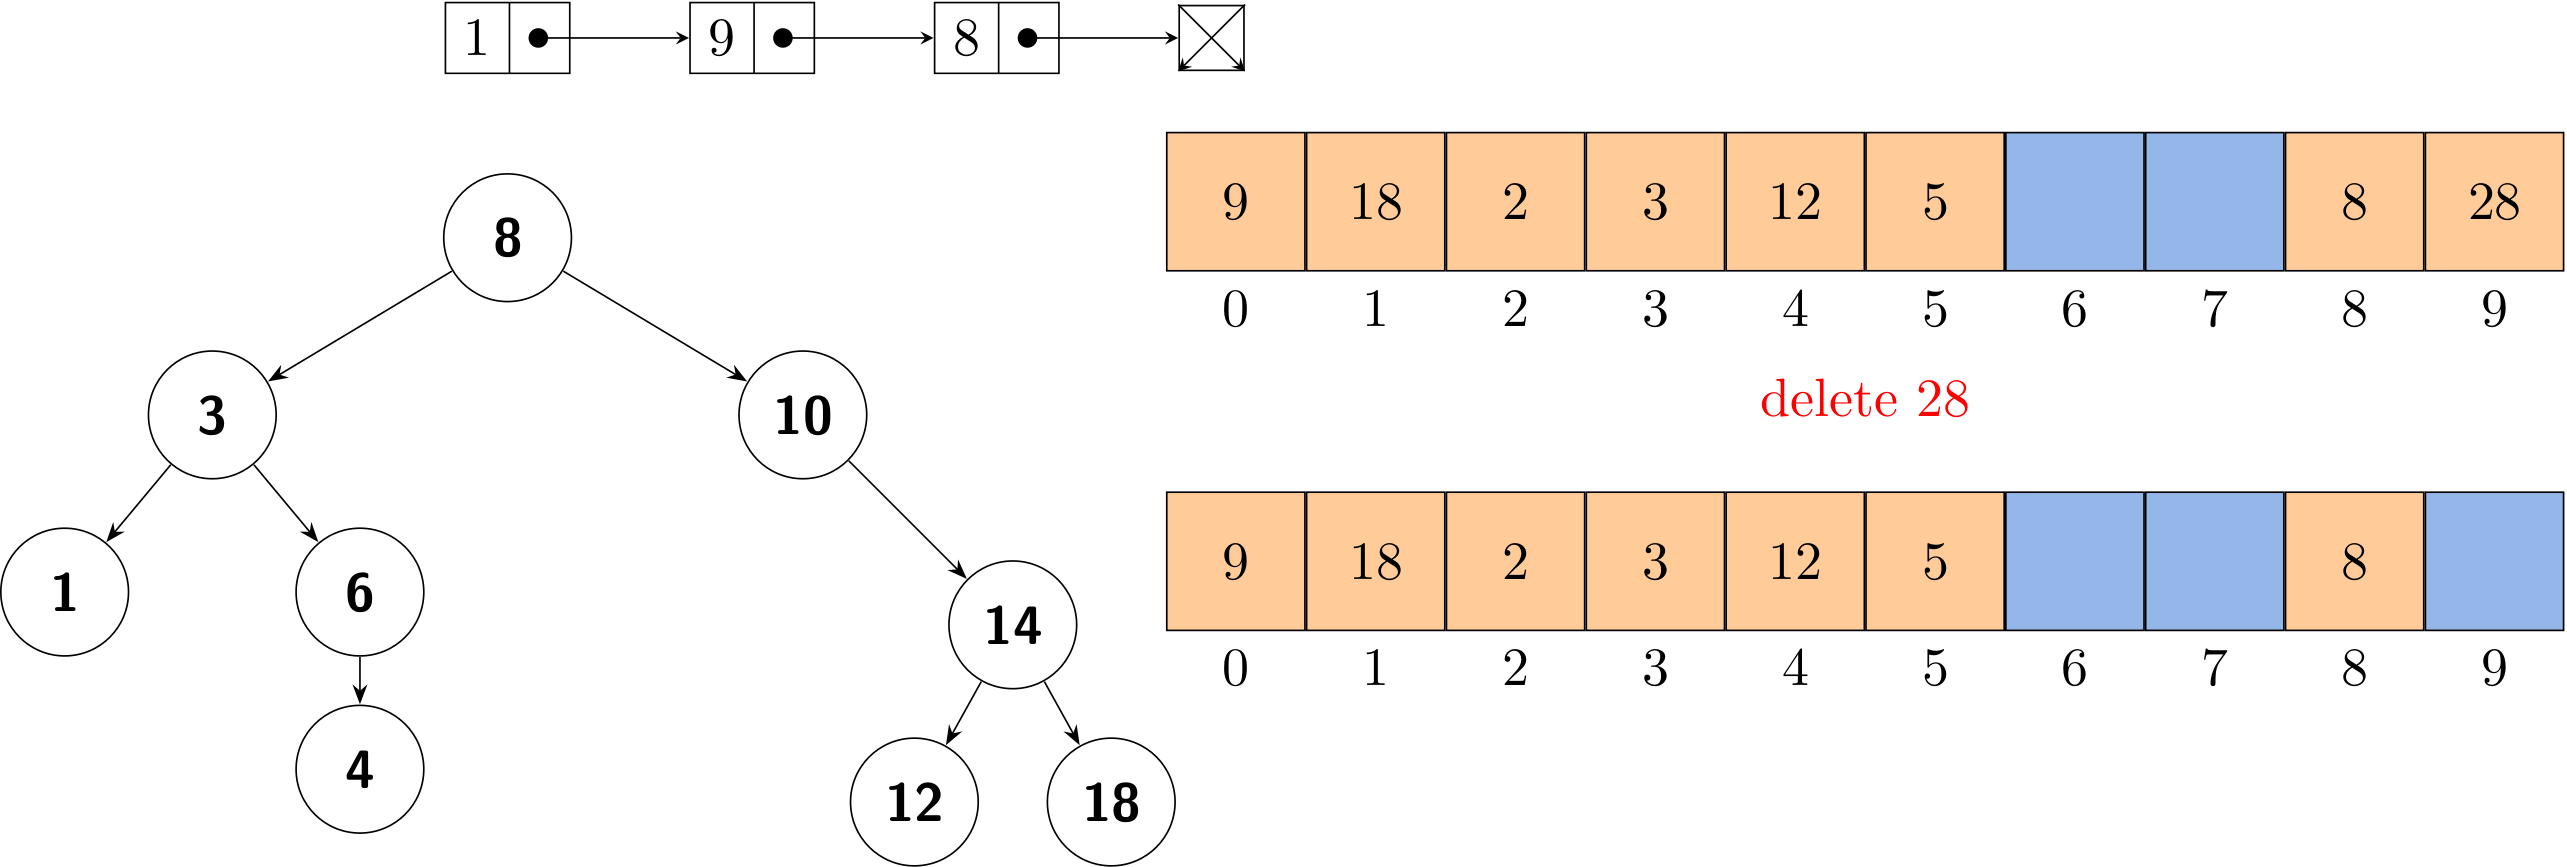
\includegraphics[height=0.6\paperheight]{cover}};
}
\begin{frame}
	\section{\textcolor{darkmidnightblue}{Built-in Data Structures}}
\end{frame}
}

\begin{frame}[fragile]
	\frametitle{Two facts}
	\begin{itemize}
		\item Even if you don't know to design your own data structures, you can still use built-in data structures to solve most daily problems.
		\item On the other hand, if you want to design your own data structures, you should know the built-in ones.
	\end{itemize}

	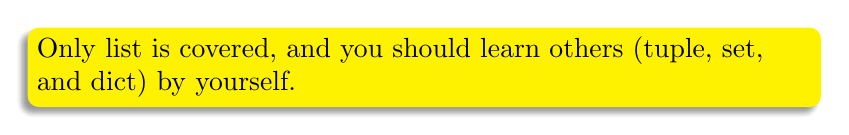
\begin{tikzpicture}
		\node[fill=yellow,blur shadow={shadow xshift=-0.5ex},
			text width=28em,anchor=south west,rounded corners]
		{Only \alert{list} is covered, and you should learn others (\alert{tuple}, \alert{set}, and \alert{dict}) by yourself.};
	\end{tikzpicture}
\end{frame}

\begin{frame}[fragile]
	\frametitle{List}
	Python's \alert{list} is similar to \alert{ArrayList} in Java, representing a mutable, ordered sequence of elements. It is created by square brackets.

	\begin{minted}[bgcolor=LightGray, fontsize=\small]{python}
num = [1, 9, 4, 2]        
num = ['1', 9, 'four', 2]
for i in num:
    print(i)
squares = [x**2 for x in range(10)]
print(3 in num)
    \end{minted}
\end{frame}

\begin{frame}[fragile]

	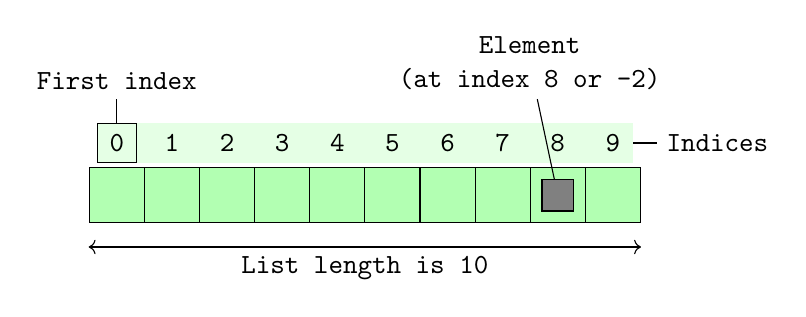
\begin{tikzpicture}[font=\ttfamily,
			array/.style={matrix of nodes,nodes={draw, minimum size=7mm, fill=green!30},column sep=-\pgflinewidth, row sep=0.5mm, nodes in empty cells,
					row 1/.style={nodes={draw=none, fill=none, minimum size=5mm}},
					row 1 column 1/.style={nodes={draw}}}]

		\matrix[array] (array) {
			0 & 1 & 2 & 3 & 4 & 5 & 6 & 7 & 8 & 9                        \\
			  &   &   &   &   &   &   &   &   & \\};
		\node[draw, fill=gray, minimum size=4mm] at (array-2-9) (box) {};

		\begin{scope}[on background layer]
			\fill[green!10] (array-1-1.north west) rectangle (array-1-10.south east);
		\end{scope}

		\draw[<->]([yshift=-3mm]array-2-1.south west) -- node[below] {List length is 10} ([yshift=-3mm]array-2-10.south east);

		\draw (array-1-1.north)--++(90:3mm) node [above] (first) {First index};
		\draw (array-1-10.east)--++(0:3mm) node [right]{Indices};
		\node [align=center, anchor=south] at (array-2-9.north west|-first.south) (8) {Element\\ (at index 8 or -2)};
		\draw (8)--(box);
	\end{tikzpicture}
	\begin{minted}[bgcolor=LightGray, fontsize=\small]{python}
# (string also supports) index and slicing
print(num[0])
print(num[0:2])
print(num[:])
print(num[-1])
print(num[2:-1])    
print(num[::-1])
    \end{minted}
\end{frame}


\begin{frame}
	You are required to know and practice at least those methods:
	\begin{enumerate}
		\item append()
		\item extend()
		\item insert()
		\item remove()
		\item pop()
		\item clear()
		\item sort()
		\item reverse()
	\end{enumerate}

	You can use \alert{len()} to get the length/size of a container (such as \alert{list} and \alert{string}).

\end{frame}

{
\usebackgroundtemplate{
	\tikz[overlay,remember picture]
	\node[opacity=0.3, at=(current page.south east),anchor=south east, yshift=2cm,xshift=4cm] {
		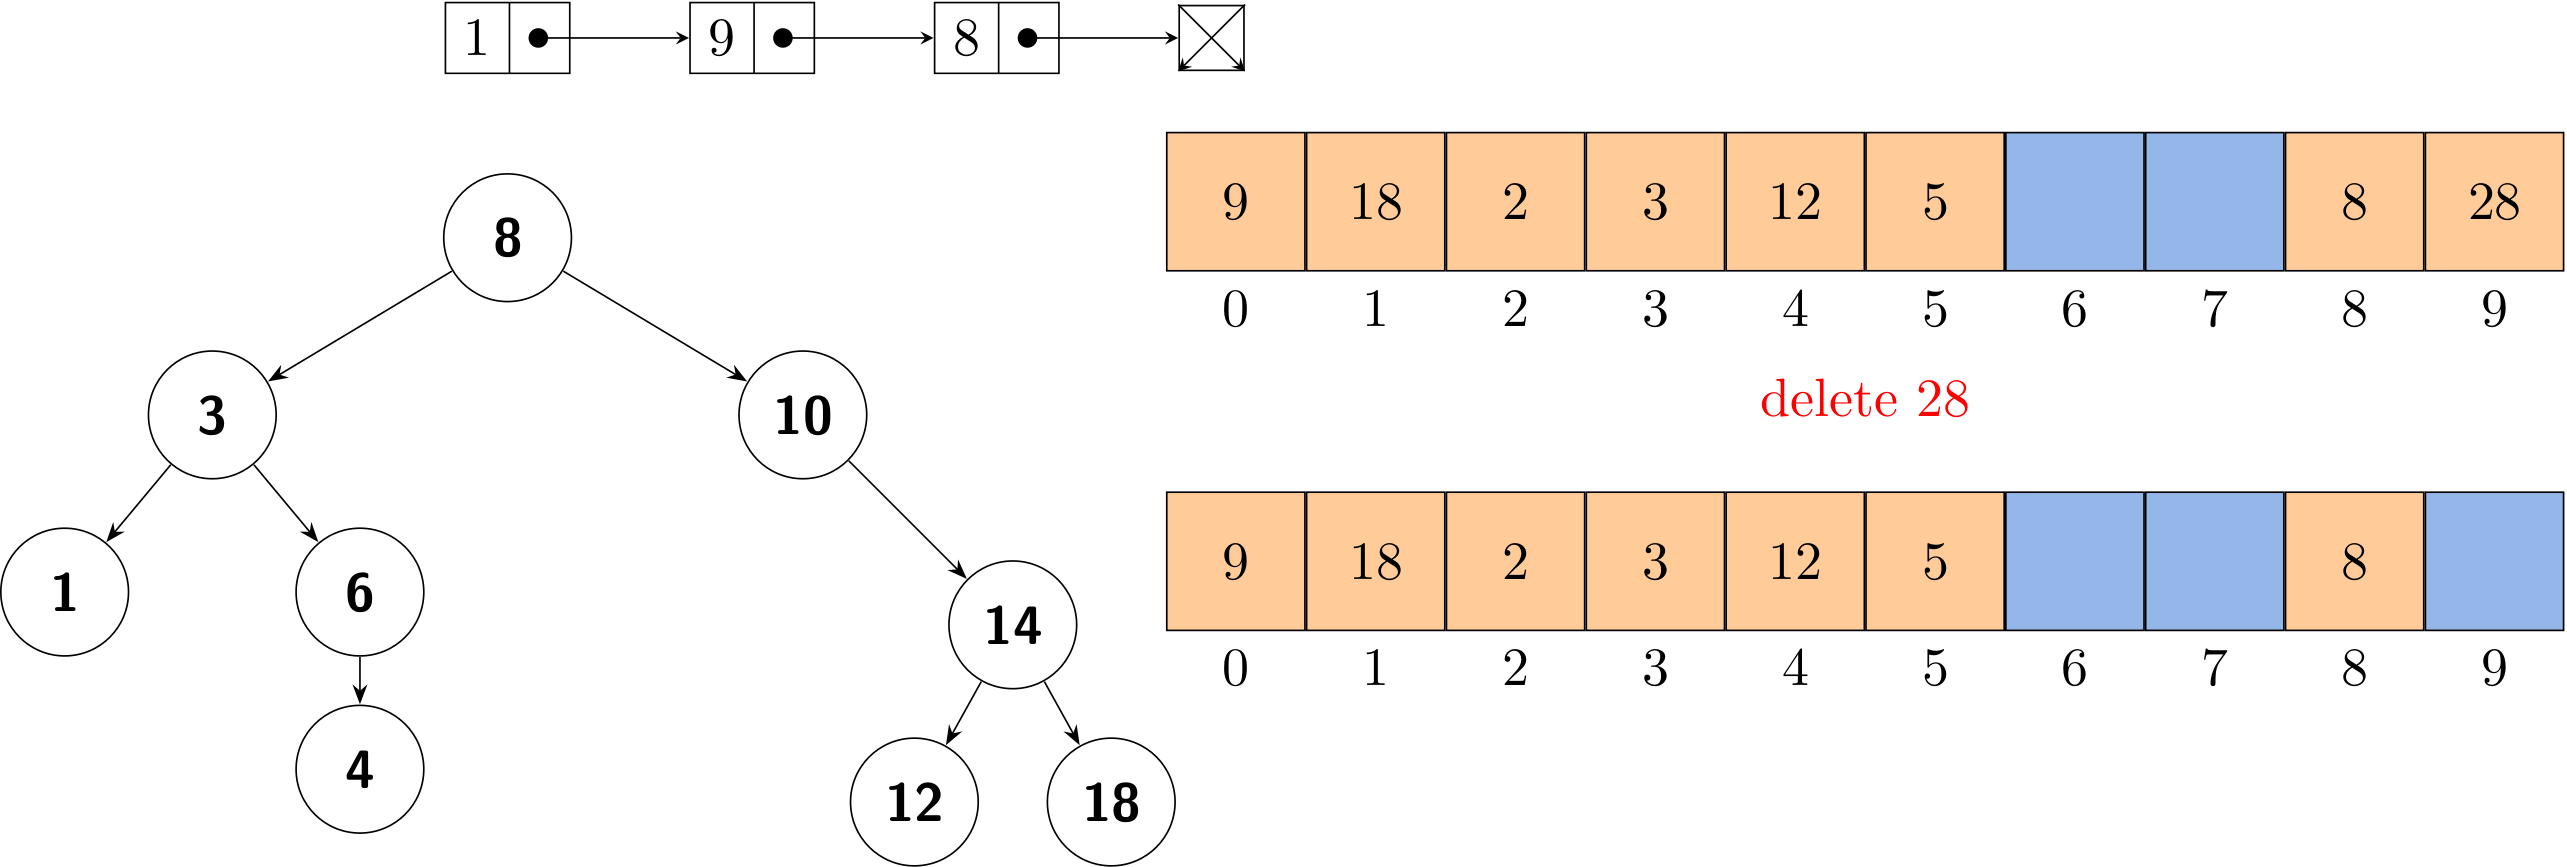
\includegraphics[height=0.6\paperheight]{cover}};
}
\begin{frame}
	\section{\textcolor{darkmidnightblue}{Why to learn data structures}}
\end{frame}
}

\begin{frame}[fragile]
	\frametitle{Review two facts}
	\begin{itemize}
		\item Even if you don't know to design your own data structures, you can still use built-in data structures to solve most daily problems.
		\item On the other hand, if you want to design your own data structures, you should know the built-in ones.
	\end{itemize}

	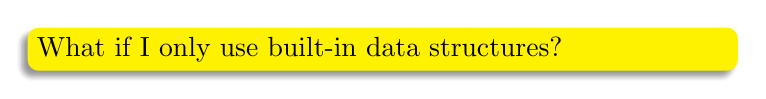
\begin{tikzpicture}
		\node[fill=yellow,blur shadow={shadow xshift=-0.5ex},
			text width=25em,anchor=south west,rounded corners]
		{What if I only use built-in data structures?};
	\end{tikzpicture}
\end{frame}

\begin{frame}[fragile]
	\frametitle{Example}
	To add a new book, which operation is better?
	\begin{minted}[bgcolor=LightGray, fontsize=\small]{python}
books = ['Gone with the wind', 'Data Structures']
books.append('Algorithms')
books.insert(0, 'Algorithms')
    \end{minted}

	Always keep \alert{efficiency} in mind.
\end{frame}

\begin{frame}[fragile]

	You can use \alert{timeit} module to test the performance of different operations.
	\begin{minted}[bgcolor=LightGray, fontsize=\small, breaklines=true]{python}
import timeit

timeit.timeit(setup='books = [i for i in range(10000)]', stmt='books.append(42)', number=100000)
timeit.timeit(setup='books = [i for i in range(10000)]', stmt='books.insert(0, 42)', number=100000)
    \end{minted}
\end{frame}

\begin{frame}
	\frametitle{Feynman: the way of learning}
	\begin{columns}
		\column{0.15\textwidth}
		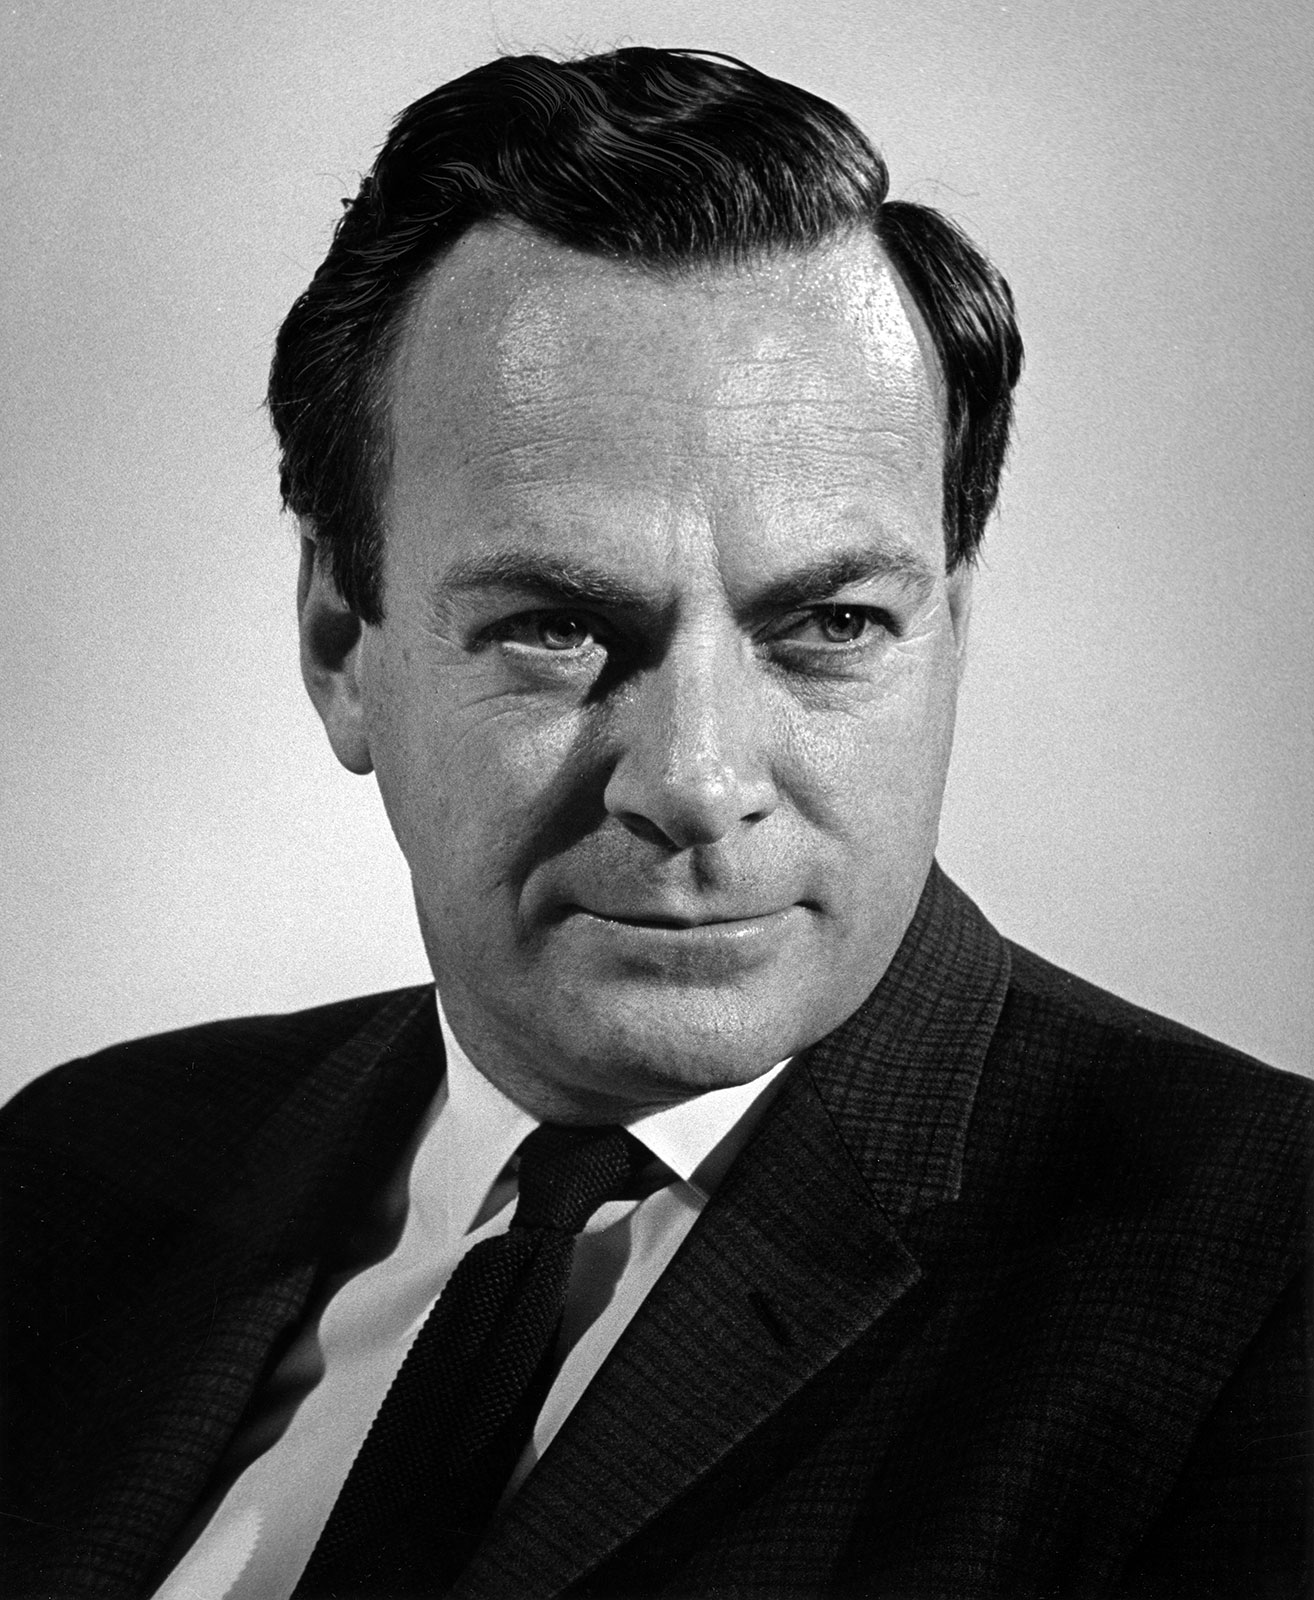
\includegraphics[height=0.5\paperheight]{week0/feynman}
		\column{0.85\textwidth}
		\begin{quote}
			``See that bird?" he says. ``Well, in Italian, it's a Chutto Lapittida. In Chinese, it's a Chung-long-tah, and in Japanese, it's a Katano Tekeda. You can know the name of that bird in all the languages of the world, but when you're finished, you'll know absolutely nothing whatever about the bird."
			(\textbf{\alert{I learned very early the difference between knowing the name of something and knowing something.}})
		\end{quote}
	\end{columns}

\end{frame}

\begin{frame}
	\section{\textcolor{darkmidnightblue}{This Week's Task}}
	\begin{itemize}
		\item Set up Python developing environment (VSCode, PyCharm, etc.)
		\item Read the official Python tutorial, and practice, practice, practice!
	\end{itemize}
\end{frame}

\begin{frame}[fragile]
	Design a class which has a list as its member variable, and has a method \alert{add()} to add a new item into it. And it also has another method implementing the following pseudocode:

	\scalebox{.7}{
		\begin{algorithm}[H]
			\caption{indexOf(a, o)}
			$n\gets a.size()$ \\
			\For{$i\gets 0$ \KwTo $n$}{
				\If{$a[i] == o$}{
					\Return{i}
				}
			}
			\Return{-1}
		\end{algorithm}
	}

\end{frame}
\end{document}
